\begin{task1}

\subsection{Task 1: Laminar Flow in a Suddenly Expanding Pipe}

%%%%%%%%%%%%%%%%% Geometry %%%%%%%%%%%%%%%%%%%%%%%%%
\subsubsection{Geometry}
The geometry of the system consists of 2 pipes of different lengths and radii joined from the ends of one another. The first and smaller pipe has a radius of 0.5cm and length 10cm while the second one has a radius of 1cm and length 25cm. In order to replicate the geometry, an axisymmetric slice from the pipe has been sketched using the Design Modeler tool of ANSYS Workbench. In this sketch which can be seen from Figure \ref{fig:sketch}, two rectangles are conjoined from the sides and the inner edge of the smaller rectangle has been trimmed to obtain the desired shape.\\

\begin{figure}[h]
    \centering
    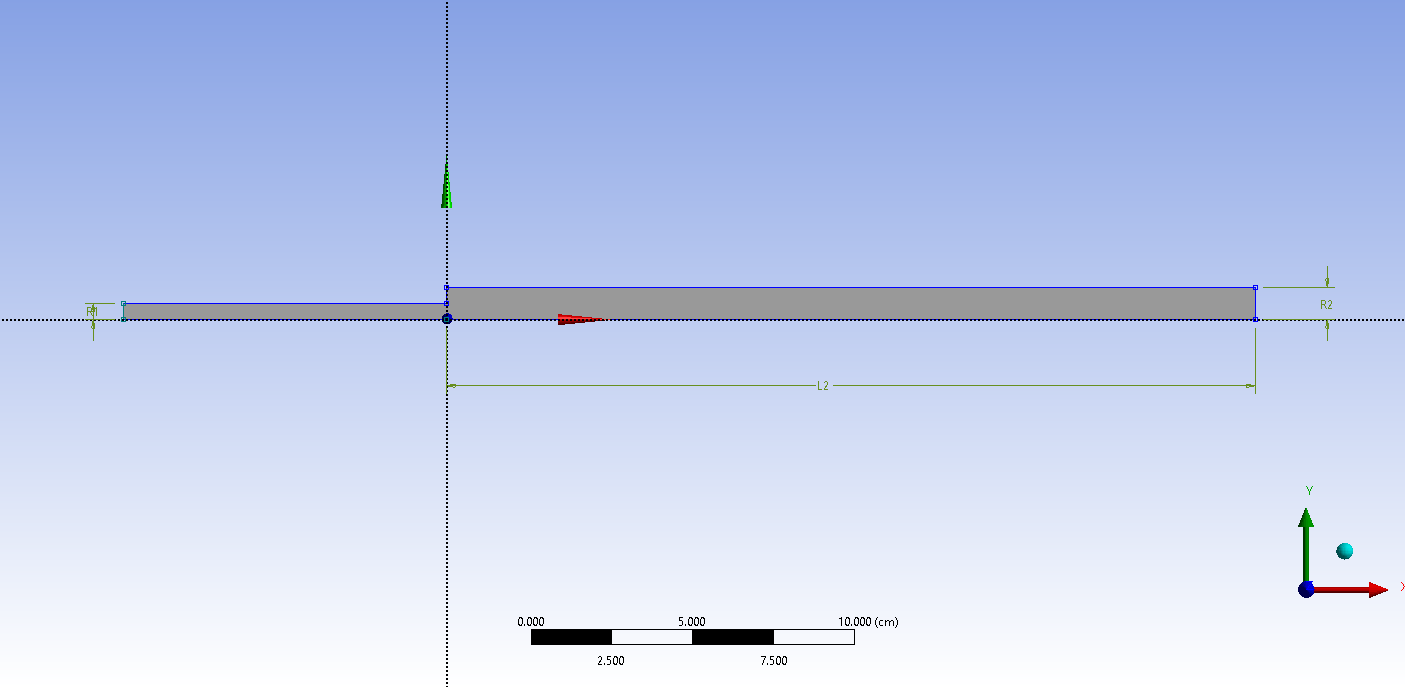
\includegraphics[width=14cm]{images/task1/sketch.png}
    \caption{Sketch of the geometry}
    \label{fig:sketch}
\end{figure}

%%%%%%%%%%% Conditions and Material Properties %%%%%%%%%%%%%%%%%%
\subsubsection{Conditions and Material Properties}
During the meshing part which will be further discussed on the following sections, named selections 
have been created and to be later used during the setup of the simulation.
CFD simulations are performed to see the behavior and change in properties of this given fluid of which its physical properties are taken to be density, $\rho = 100 \frac{kg}{m^{3}}$ and dynamic viscosity $\mu = 0.01 \frac{kg}{ms}. $\\

\noindent For this task, different values like the inlet velocity, density, inlet diameter and viscosity are chosen carefully to keep the Reynolds number of the flow under 2300, which ensures a laminar flow. The inlet velocity is set to be 0.554 m/s. The Reynolds number for this setup is calculated as follows:
\begin{equation} \label{eq:reynolds}
     Re = \frac{\rho * V_1 * (2R_1)}{\mu} = 55.4
\end{equation}
\\

\noindent The axisymmetric condition is selected with the lowermost edge being the symmetry axis and the remaining edges excluding the inlet and outlet are selected to be walls. Meaning that boundary conditions can be seen from Figure \ref{fig:boundary} where red lines show the inlet, yellows the outlet, greens the walls and the blue representing the symmetry axis. \\


\begin{figure}[h]
    \centering
    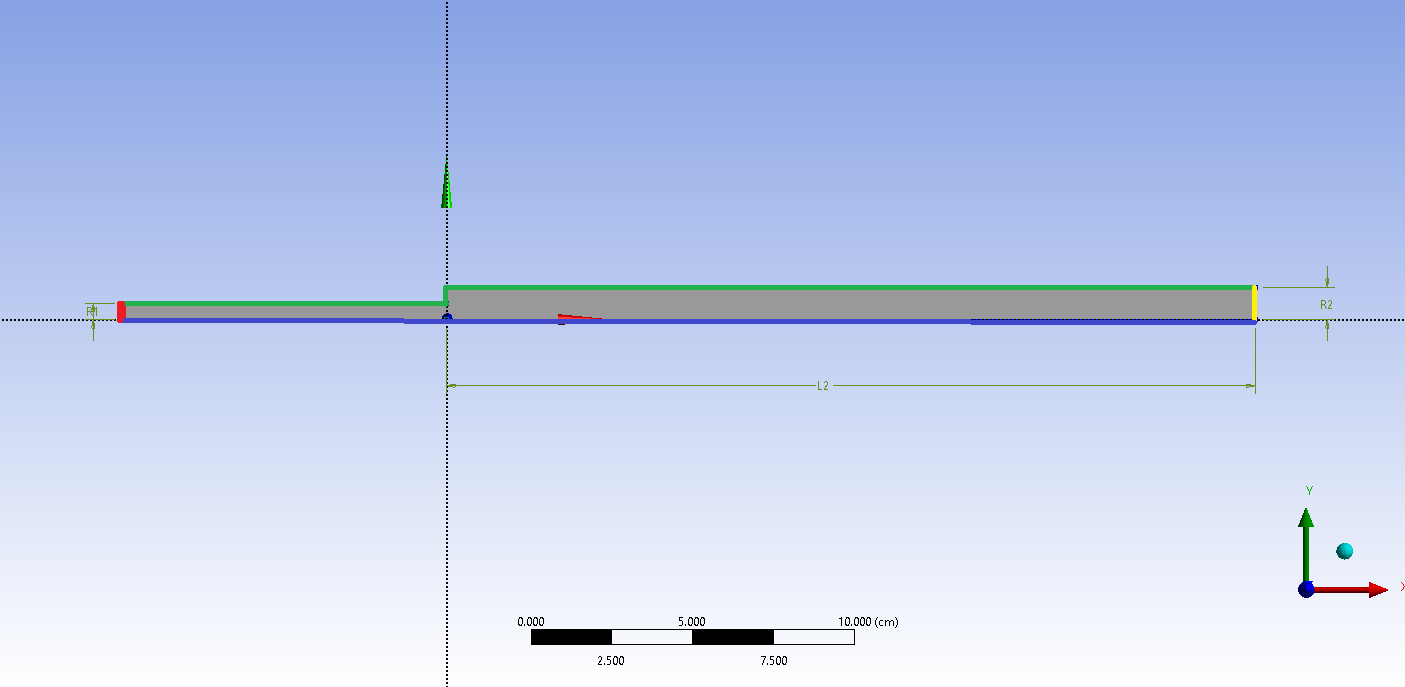
\includegraphics[width=15cm]{images/task1/sketch_paint.png}
    \caption{Boundary Conditions}
    \label{fig:boundary}
\end{figure}

\noindent When making the calculations, the laminar, axisymmetric flow parameters have been selected from the solver settings to represent the system properly and a Least Square based calculation is run.












%%%%%%%%%%%%%%%%%%%  %%%%%%%%%%%%%%%%%%%%



\end{task1}